\chapter{IMSRG(3) for the pairing Hamiltonian}\label{app:pairing_hamiltonian_imsrg3}

The pairing Hamiltonian is given by
\begin{equation}\label{eq:pairing_hamiltonian}
    H = \delta \sum_{p\sigma} (p - 1) \crea{p\sigma} \annih{p\sigma}
    - \frac{g}{2} \sum_{p q} \crea{p+}\crea{p-} \annih{q-} \annih{q+}\,,
\end{equation}
where we have equally-spaced two-fold degenerate levels indexed by the quantum number $p$
and an attractive (for $g > 0$) pairing interaction.
Cooper first considered this Hamiltonian in 1956~\cite{Coop56pairing_hamiltonian},
which led to the successful Bardeen-Cooper-Schreifer (BCS) theory of superconductivity~\cite{Bard57bcs}.
The exact eigenvalues of the pairing Hamiltonian were given by Richardson in 1963,
where the solutions are obtained via the solution of the non-linear coupled Richardson equations~\cite{Rich63pairing_hamiltonian}.

We focus on a restricted case where $p=1,\ldots,4$ and $\delta=1\mev$,
and we vary the strength of the pairing interaction $g$.
We are interested in the ground state of four fermions,
for which our reference state is the state with the two lowest levels completely filled,
\begin{equation}\label{eq:pairing_hamiltonian_reference}
    \refgnd = \crea{2-}\crea{2+}\crea{1-}\crea{1+}\ket{0}\,.
\end{equation}
This system has a couple of useful properties:
First, the number of single-particle states is only eight,
making the IMSRG(3) calculation relatively tractable.
Additionally, one can increase the number of levels $p_{\text{max}}$ easily
to get a handle on the performance for larger single-particle basis sizes.
Second, in addition to the available exact solution,
this system is easy to construct and diagonalize in the basis
of the reference state and its particle-hole excitations,
\begin{equation}
    \{\refgnd, \refhp{ij}{ab}, \refhp{ijkl}{abcd} \}\,,
\end{equation}
where the odd number particle-hole excitations do not contribute
as Eq.~\eqref{eq:pairing_hamiltonian} only couples pairs.
This makes it easy to obtain an exact solution with which to compare the IMSRG(2)
and IMSRG(3) solutions.
Finally, after normal ordering the Hamiltonian with respect to our reference state,
we find that $\hnoone$ is diagonal,
meaning our reference state is the canonical Hartree-Fock reference state
with the Hartree-Fock energy $\hnozero=E_{\text{HF}}=2 - g$.
This means the IMSRG evolution must only bring in correlation corrections to the energy
without needing to overcome any reference state deficiencies.

\begin{figure}[t]
    \centering
    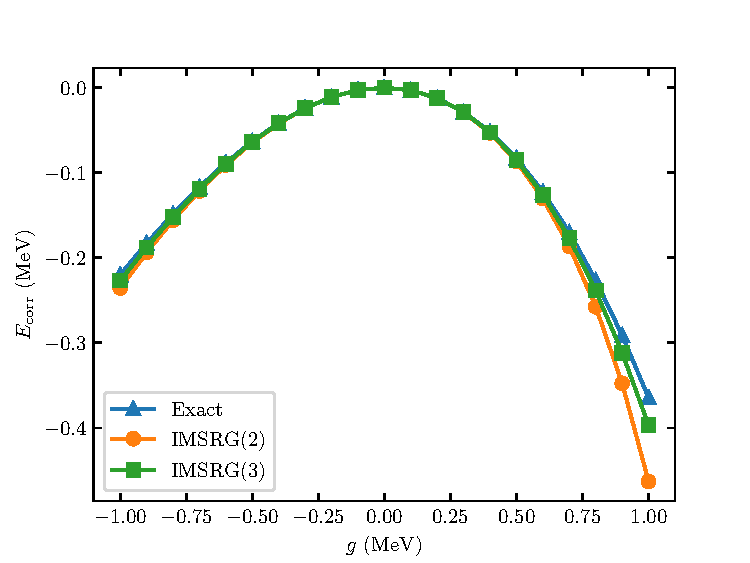
\includegraphics[width=0.9\textwidth]{thesis/doc/images/pairing_ham_imsrg3.pdf}
    \caption[
        The correlation energy $E_{\text{corr}}$ for the solution of the pairing Hamiltonian
        obtained via exact diagonalization,
        IMSRG(2), and IMSRG(3)
        for $-1 \le g \le 1$.
    ]{
        The correlation energy $E_{\text{corr}}$ for the solution of the pairing Hamiltonian
        obtained via exact diagonalization,
        IMSRG(2), and IMSRG(3)
        for $-1 \le g \le 1$.
        Exact diagonalization results obtained using code published with Ref.~\cite{Liet16lecnotesphysics}.
    }\label{fig:pairing_hamiltonian_fig}
\end{figure}

Thus, we are interested in the correlation energy obtained by the IMSRG(2) and IMSRG(3) solutions,
defined as
\begin{equation}
    E_{\text{corr}} \equiv E(s \rightarrow \infty) - E(s= 0)\,.
\end{equation}
This is plotted in Fig.~\ref{fig:pairing_hamiltonian_fig} for $-1 \le g \le 1$.
We find generally good agreement between the IMSRG correlation energy
and the exact correlation energy,
with the exception of the region for $0.5 \le g \le 1$.
Here, the IMSRG(3) calculation improves upon the relatively large error in the IMSRG(2)
correlation energy,
which in Ref.~\cite{Herg16imsrglecnotes}
was explained as being due to an overcounting in the fourth-order diagrams in MBPT
by a factor of 1/2 present in the IMSRG(2) truncation.
It seems that this overcounting at fourth-order is lifted in the IMSRG(3).
We note here that our results for IMSRG(2) match exactly with those from Ref.~\cite{Herg16imsrglecnotes}.
